\large{
Avendo analizzato nel capitolo precedente le primitive di interazione per la visualizzazione di un grafo clusterizzato ora si tratterà delle operazioni di semplificazione, frutto di anni di ricerche(~\cite{10.1007/978-3-642-11805-0_8},~\cite{DBLP:journals/corr/abs-1808-07437},~\cite{pipe2018},~\cite{angelini_et_al:LIPIcs:2016:6781},~\cite{10.1093/comjnl/bxw035},~\cite{10.1007/3-540-45848-4_5}). Data la complessità nel definire se in tempo polinomiale è possibile dato un grafo clusterizzato costruire un disegno planare clusterizzato, si sono realizzate delle riduzioni polinomiali che semplificano il problema.
\section{Riduzione polinomiale}
Prima di poter analizzare i progressi svolti nell'ambito della semplificazione dei grafi clusterizzati è necessario fornire la definizione di riduzione polinomiale poiché sarà poi ampiamente utilizzata nel capitolo essendo le due semplificazioni riportate di seguito frutto appunto di riduzioni polinomiali.
La \textbf{Riduzione polinomiale} tra problemi è definibile come segue:\\
\newline
\begin{center}
	\textit{Un problema $\textbf{P1}$ si riduce in tempo polinomiale a un problema $\textbf{P2}$, in formule $P1<=_pP2$, se esiste una funzione $f$ calcolabile in tempo polinomiale tale che $X$ è una soluzione di $P1$ \textbf{se e solo se} $f(X)$ è una soluzione di $P2$}
\end{center}
In altre parole un problema \textbf{A} si riduce polinomialmente ad un problema \textbf{B} se, data un’istanza $a$ di A, è possibile costruire in tempo polinomiale un’istanza $b$ del problema B tale che $a$ è affermativa se e solo se $b$ è affermativa.Si noti inoltre che se un problema A si riduce ad un problema B allora risolvendo efficientemente B siamo in grado di risolvere anche A. Avendo dato le definizioni di classi di complessità $P$ e $NP$ , un problema A è definibile \textbf{NP-completo} se 
$$A \in NP e B<=_pP \forall B\in NP$$
 
\section{Flat clustered-planarity}
%professor patrignani da citare
Mediante il lavoro svolto dal professor Maurizio Patrignani nel 2018 si visto che tramite una riduzione polinomiale definibile come:
\begin{center}
	\textit{C\_planarity $<=_p$ Flat C\_planarity}
\end{center} 
 il \textit{c-graph} $C$ definito come $C(G,T)$  può essere ridotto in una istanza \textbf{equivalente} $C_f(G_f,T_F)$ in cui $T_f$ è flat.
Definendo che una istanza $C(G,T)$ di un c-graph con $n$ vertici e $c$ cluster può essere ridotta in tempo $O(n+c)$ in una istanza equivalente in cui $T$è omogeneo, la $r(T)$ definita come la radice dell'albero ha almeno due figli e $h(T)<=n-1$,
è possibile ottenere in un tempo $O(n+c)$ che $T$ è omogeneo e $S(T)\in O(n)$.
Come visto dalla definizione di riduzione polinomiale risolvendo questo problema definito \textbf{Flat Clustered planarity} allora si risolverebbe anche il problema Clustered Planarity essendo polinomialmente riducibile al primo.
\newpage
\begin{figure}[!htb]
	\begin{center}
		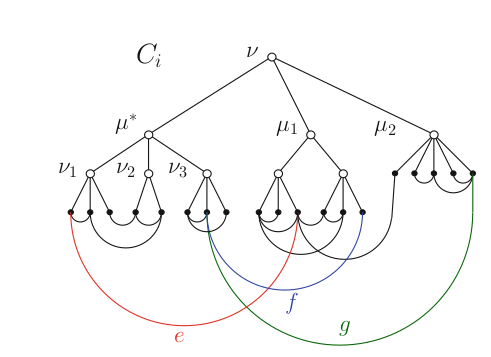
\includegraphics[width=0.8 \linewidth]{figure/preFlat}
	\end{center}
	\caption{$C_i$ con albero di inclusione $T$ omogeneo \label{fig:preFlat}}
\end{figure} 
La riduzione consiste in una sequenza di trasformazioni di $C$ = $C_0$ in $C_1$, $C_2$,. . . , $C_{S(T)} = C_f$, dove:
$$C_i = <G_i, T_i>$$
$$i = 0, 1,. . . , S(T)$$
in cui: $C_i$ ha un albero di inclusione $T_i$ omogeneo; ogni trasformazione richiede tempo polinomiale $O(n)$; $S(T)$ è definito come la dimensione dell'albero di inclusione $T$, ovvero il numero di nodi superiori di $T$ diversi dalla radice.\\
Prendendo, come mostrato in figura \figurename~\ref{fig:preFlat}, un grafo clusterizzato $C_i$ nella sua rappresentazione ad albero "layered" è possibile vedere come esso rispetti le condizioni imposte in quanto l'albero di inclusione $T_i$ risulta omogeneo avendo definito in precedenza che un albero è omogeneo se e solo se tutti i suoi nodi sono nodi omogenei ovvero se tutti i figli di quel nodo sono foglie o sono nodi interni. È possibile dunque costruire $C_{i+1} = <G_{i+1},T_{i+1}>$ come segue:
\begin{itemize}
	\item \textbf{$ G_{i+1} $} è ottenuto introducendo $\forall e=<u,v>$ di $\mu^*$, dove $\mu^*$ è un cluster ed $e$ è un arco inter-cluster, ovvero un arco si connessione tra i due nodi $u$ e $v$ appartenenti a cluster diversi, due nuovi vertici definiti $e_\chi$ ed $e_\varphi$ e sostituendo $e$ con un percorso $$(u, e_\chi)(e_\chi, e\varphi) (e_\varphi, v)$$
	\item \textbf{$T_{i+1}$} è ottenuto rimuovendo $\mu^*$, attaccando i suoi figli $v_1, v_2,. . . , v_h$ direttamente al cluster radice $v$ e aggiungendo ad esso due nuovi figli $\chi$ e $\varphi$, i quali conterranno tutti i vertici introdotti nella sostituzione di un arco inter-cluster di  $\mu^*$ con un sentiero.
\end{itemize}
\begin{figure}[!htb]
	\begin{center}
		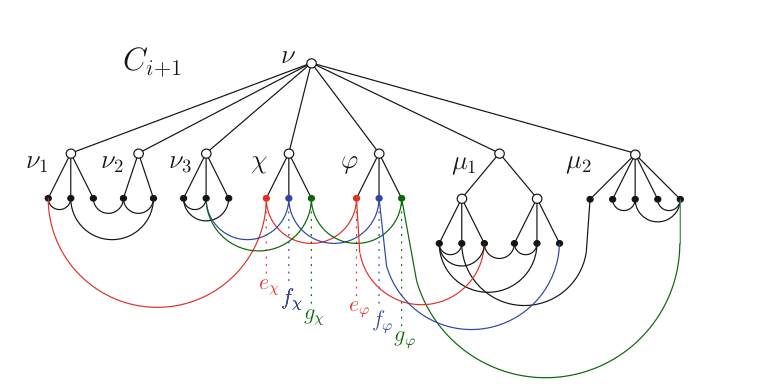
\includegraphics[width=1 \linewidth]{figure/postFlat}
	\end{center}
	\caption{$C_{i+1}$ ottenuto dopo parte del processo di riduzione \label{fig:postFlat}}
\end{figure}
Ottenendo in questo modo la rappresentazione mostrata nella figura \figurename~\ref{fig:postFlat}.
\newpage
Iterando la costruzione $\forall i$ si arriva ad avere un albero di inclusione $T$ di profondità $d=2$ in cui ogni cluster $c$ è un nodo interno dell'albero ed ogni foglia è rappresentata da un nodo dell'underlying graph, ovvero $T$ flat e nel grafo non si è persa conoscenza o connessione tra i nodi che risulteranno essere connessi comunque tra loro.
\begin{figure}[!htb]
	\begin{center}
		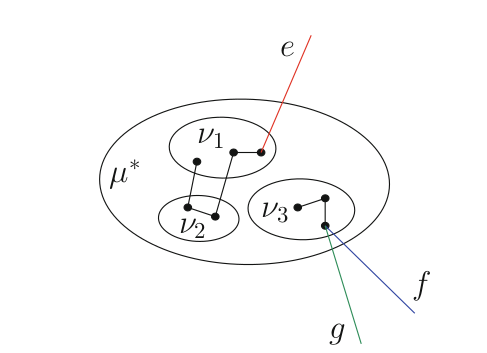
\includegraphics[width=1 \linewidth]{figure/dettaglioCluster}
	\end{center}
	\caption{Dettaglio del cluster $\mu^*$ con rappresentazione Spring-enbedding \label{fig:dettaglioCluster}}
\end{figure}
\newline
È inoltre possibile visualizzare la riduzione senza dover necessariamente utilizzare l'albero di inclusione. Partendo da una rappresentazione node-link, utilizzando il modello Force-Directed,  del grafo cluterizzato ed in particolare soffermandosi solamente sul dettaglio del cluster $\mu^*$ di livello $l>2$, visualizzato in \figurename~\ref{fig:dettaglioCluster}, è possibile comunque eseguire la riduzione in quanto indipendente dal tipo di visualizzazione. Seguendo i passi visti prima per la costruzione del grafo clusterizzato $C_{i+1} = <G_{i+1},T_{i+1}>$, con un modello Node-link si otterrà una visualizzazione simile a quella mostrata nella \figurename~\ref{fig:flatSpring}. Come si nota i cluster aggiunti $\chi$ e $\varphi$, che vanno a sostituire l'originale $\mu^*$, hanno una forma non più circolare ma ad anello. Questi cluster $\chi$ e $\varphi$ per permettere una maggiore copertura per quanto riguarda i possibili nodi $e_\chi$ ed $e_\varphi$ circonderanno i cluster che in precedenza appartenevano alla lista dei figli di $\mu^*$. Questo fa in modo di avere una visualizzazione a grafo non più puramente node-link ma è comunque possibile applicate le forze in gioco per poter raggiungere un equilibrio nel caso di un modello force-directed. Gli anelli dei cluster $\chi$ e $\varphi$ sono solo una delle possibili visualizzazioni in quanto essi possono anche esser rappresentati allo stesso modo dei cluster.
\begin{figure}[!htb]
	\begin{center}
		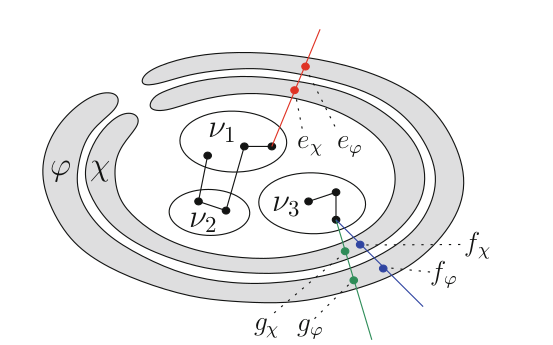
\includegraphics[width=1.1 \linewidth]{figure/flatSpring}
	\end{center}
	\caption{Cluster $\mu^*$ dopo la riduzione con rappresentazione semi Spring-enbedding \label{fig:flatSpring}}
\end{figure}
\newline
Per completezza si riportano le caratteristiche saltate in questa sezione fino ad ora che rappresentano ovvietà non specificate:
\begin{itemize}
	\item Se l'albero di inclusione $T_i$ è omogeneo, allora $T_{i + 1}$ è omogeneo, in quanto ogni nodo interno non avrà comunque nodi cluster e non al suo interno dopo la riduzione.
	\item $S(T_{i+1})= S(T_i)-1$, ricordando che $S(T)$ è la dimenzione dell'albero $T$
	\item il grafo clusterizzato $C_f = C_{S(T)}$ è flat.
\end{itemize} 
Per concludere si può dunque denotare che\\ 
\begin{center}
	$C_i(G_i , T_i )$ è un disegno planare \textbf{c-planar} di un grafo clusterizzato se e solo se anche $C_{i+1}(G_{i+1} , T_{i+1} )$ è un disegno planare 
\end{center}
\section{Pipe clustered planarity}
È possibile la realizzazione anche della riduzione in disegno planare Pipe che sarà introdotta di seguito e la cui composizione, partendo da un disegno planare Flat fino alla costruzione del disegno c-planare Pipe, è mostrata nella  \figurename~\ref{fig:composizionePipe}.
\begin{figure}[!htb]
	\begin{center}
		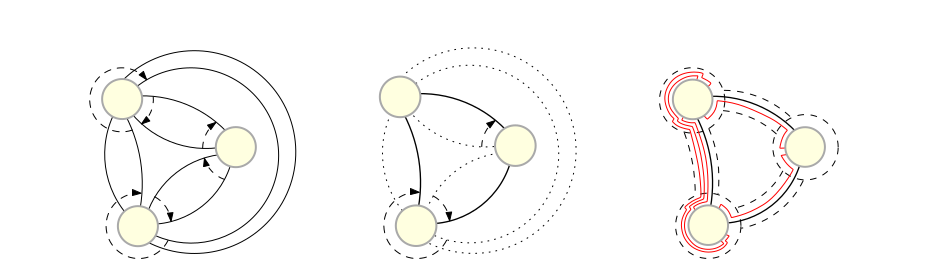
\includegraphics[width=0.95 \linewidth]{figure/composizionePipe}
	\end{center}
	\caption{creazione di un disegno c-planare Pipe partendo da un disegno c-planare Flat \label{fig:composizionePipe}}
\end{figure}
\newline
Avendo già definito i concetti di grafo clusterizzato, disegno planare, riduzione polinomiale e tutto ciò che ne concerne definiamo adesso il concetto di pipe su cui si basa la riduzione.
Sia $\Gamma(C)$ un disegno c-planare di un c-grafico $C$. Per ogni cluster $\mu_i$ di $C$, il disegno $\Gamma$ induce un ordine $O_{orario}(\mu_i)$ in senso orario dei bordi tra cluster di $\mu_i$, ovvero l'ordine circolare in cui si incontrano i bordi tra i cluster di $\mu_i$ mentre si attraversa in senso orario il limite di $R(\mu_i)$ in $\Gamma$. Allo stesso modo, definiamo l'ordinamento antiorario $O_{antiorario}(\mu_i)$ dei bordi tra cluster di $\mu_i$. Un disegno c-planare Pipe $\Gamma_p(C)$ di un grafo flat $C(G, T)$ è un disegno c-planare di $C$ tale che, per qualsiasi coppia di cluster vicini $\mu_i$ e $\mu_j$, esiste un semplice regione chiusa $R(\mu_i, \mu_j)$, detta Pipe, che tocca $R(\mu_i)$ e $R(\mu_j)$ e che contiene esclusivamente la porzione dei bordi inter-cluster in $E(\mu_i, \mu_j)$ all'esterno di $R(\mu_i)$ e $R(\mu_j)$.\\
Viene di seguito data la condizione necessaria affinché una istanza flat possa essere ridotta ad una pipe:\\
\begin{center}
	\textit{Il grafo clusterizzato $C$ ammette un disegno c-planare $\tau(C)$ tale che per $\forall E(\mu_i,\mu_j)$ arco di $C$, i bordi di $E(\mu_i,\mu_j)$ compaiono consecutivamente nell'ordine orario $O_{orario}(\mu_i)$ nello stesso ordine in cui appaiono consecutivamente nell'ordine $O_{antiorario}(\mu_j)$.}\newline
\end{center}
Definita questa condizione è possibile eseguire una riduzione di una istanza pipe clustered planarity in una flat clustered planarity e viceversa.
\newpage
Definita $C_p$ una istanza di pipe clustered planarity e $C_f$ una di flat clustered planarity è dunque possibile definire la riduzione Pipe C\_planarity $<=_p$ Flat C\_planarity e viceversa come segue:
\begin{center}
	\textit{Se $C_p= (G_p, T_p)$ è un'istanza positiva di pipe clustered planarity allora $C_f (G_f, T_f)$ è un'istanza positiva di Flat clustered planarity}
\end{center}
La dimostrazione si basa sulla costruzione di un disegno c-planare $\tau(C_f)$ a partire da un disegno c-planare pipe $\tau(C_p)$ come mostrato nella \figurename~\ref{fig:flatVsPipe}.
\begin{figure}[!htb]
	\begin{center}
		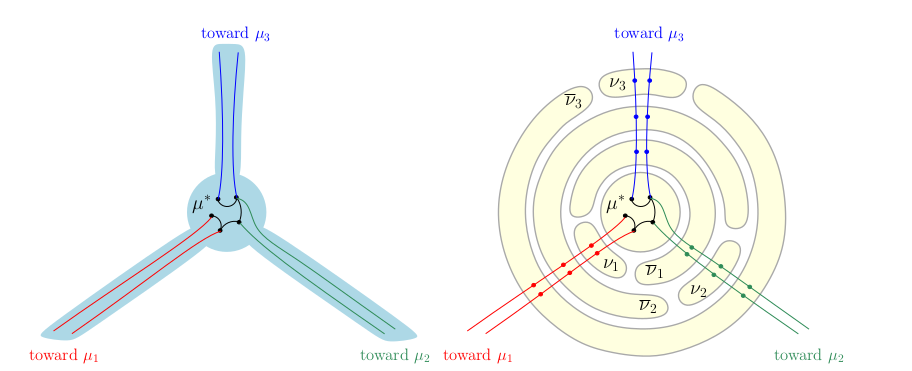
\includegraphics[width=1 \linewidth]{figure/flatVsPipe}
	\end{center}
	\caption{Dettaglio di un cluster in c-planare Pipe ed in c-planare Flat \label{fig:flatVsPipe}}
\end{figure}

}
